% Prezentare CFAR-STFT Detecția Radarului
% Autori: Ingrid Corobana, Teodora Nae
% Compilare: pdflatex presentation_ro.tex (de 2 ori pentru TOC)

\documentclass[12pt,aspectratio=169]{beamer}

\usepackage[utf8]{inputenc}
\usepackage[romanian]{babel}
\usepackage{amsmath}
\usepackage{amssymb}
\usepackage{graphicx}
\usepackage{tikz}
\usepackage{xcolor}
\usepackage{hyperref}
\usepackage{booktabs}
\usepackage{multicol}

% Tema și culori
\usetheme{Madrid}
\usecolortheme{default}

\definecolor{stftblue}{RGB}{66, 133, 244}
\definecolor{cfarorange}{RGB}{255, 152, 0}
\definecolor{dbscangreen}{RGB}{76, 175, 80}
\definecolor{darkblue}{RGB}{25, 50, 100}
\definecolor{ipixpurple}{RGB}{156, 39, 176}

\setbeamercolor{structure}{fg=darkblue}
\setbeamercolor{alerted text}{fg=cfarorange}
\setbeamercolor{example text}{fg=dbscangreen}

% Calea pentru imagini
\graphicspath{{../results/ipix_figures/}{../results/animations/}{images/}}

\title[CFAR-STFT]{Analiza semnalelor radar în prezența ecourilor marine}
\subtitle{Abordare CFAR-STFT cu adaptări pentru date reale}
\author[Corobana, Nae]{Ingrid Corobana \and Teodora Nae}
\date{Procesarea Semnalelor -- 2026}
\institute[FMI]{Universitatea din București\\Facultatea de Matematică și Informatică\\[0.3em]
Coordonator: Prof. Dr. Cristian Rusu}

\begin{document}

% ============================================================================
% SLIDE 1: TITLU
% ============================================================================
\begin{frame}
\titlepage
\end{frame}

% ============================================================================
% SECȚIUNEA 1: INTRODUCERE
% ============================================================================
\section{Introducere}

\begin{frame}{Problema și Soluția CFAR-STFT}
\begin{columns}[T]
\column{0.5\textwidth}
\textbf{Sea Clutter}:
\begin{itemize}
    \item Ecouri radar de la suprafața mării
    \item Non-Gaussian (spike-uri frecvente)
    \item Ascunde target-uri mici
\end{itemize}

\vspace{0.5em}
\textbf{Pipeline CFAR-STFT}:
\begin{enumerate}
    \item STFT $\rightarrow$ spectrogramă
    \item CFAR 2D $\rightarrow$ detecție adaptivă
    \item DBSCAN $\rightarrow$ clustering
    \item Dilatare + iSTFT $\rightarrow$ reconstrucție
\end{enumerate}

\column{0.5\textwidth}
\begin{figure}
\includegraphics[width=\textwidth]{ipix_seaclutter_explanation.png}
\end{figure}
\end{columns}
\end{frame}

% ============================================================================
% SECȚIUNEA 2: GOCA-CFAR
% ============================================================================
\section{GOCA-CFAR 2D}

\begin{frame}{GOCA-CFAR 2D -- Detecție Adaptivă}
\begin{columns}[T]
\column{0.5\textwidth}
\centering
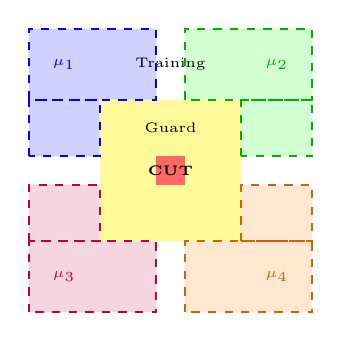
\begin{tikzpicture}[scale=0.45]
    % Training regions (mu_k) = ONLY training cells (exclude Guard + CUT).
    % Draw as "L-shape" (outer quadrant minus guard overlap) for clarity.
    \path[fill=blue!18, even odd rule] (-4,0.4) rectangle (-0.4,4) (-2,0.4) rectangle (-0.4,2);
    \path[fill=green!18, even odd rule] (0.4,0.4) rectangle (4,4) (0.4,0.4) rectangle (2,2);
    \path[fill=purple!16, even odd rule] (-4,-4) rectangle (-0.4,-0.4) (-2,-2) rectangle (-0.4,-0.4);
    \path[fill=orange!18, even odd rule] (0.4,-4) rectangle (4,-0.4) (0.4,-2) rectangle (2,-0.4);

    % Guard cells (excluded from mu_k)
    \fill[yellow!40] (-2,-2) rectangle (2,2);

    % CUT
    \fill[red!60] (-0.4,-0.4) rectangle (0.4,0.4);
    
    \node at (0,0) {\tiny\textbf{CUT}};
    \node at (0,1.2) {\tiny Guard};
    \node at (0,3) {\tiny Training};
    
    % GOCA quadrants
    % L-shape outlines (training only, fara guard)
    \draw[blue, dashed, thick] (-4,0.4) rectangle (-2,2);
    \draw[blue, dashed, thick] (-4,2) rectangle (-0.4,4);
    \draw[green!70!black, dashed, thick] (2,0.4) rectangle (4,2);
    \draw[green!70!black, dashed, thick] (0.4,2) rectangle (4,4);
    \draw[purple, dashed, thick] (-4,-2) rectangle (-2,-0.4);
    \draw[purple, dashed, thick] (-4,-4) rectangle (-0.4,-2);
    \draw[orange!80!black, dashed, thick] (2,-2) rectangle (4,-0.4);
    \draw[orange!80!black, dashed, thick] (0.4,-4) rectangle (4,-2);
    
    \node[blue, font=\tiny] at (-3.0,3.0) {$\mu_1$};
    \node[green!70!black, font=\tiny] at (3.0,3.0) {$\mu_2$};
    \node[purple, font=\tiny] at (-3.0,-3.0) {$\mu_3$};
    \node[orange!80!black, font=\tiny] at (3.0,-3.0) {$\mu_4$};
\end{tikzpicture}

\vspace{0.3em}
{\scriptsize \textit{Notă:} excludem o „cruce” (buffer) între cadrane pentru a evita ridge/sidelobe-uri pe axe.}

\vspace{0.2em}
{\footnotesize \textbf{Parametri IPIX:} $N_G = 3$, $N_T = 12$, $P_f = 0.001$ \textit{(semnificativ mai mic decat in paper!)}}

\column{0.5\textwidth}
\textbf{GOCA = Greatest-Of Cell Averaging}
\begin{align*}
\hat{Z} &= \max(\mu_1, \mu_2, \mu_3, \mu_4) \\
T &= R \cdot \hat{Z} \\
R &= N_T (P_f^{-1/N_T} - 1)
\end{align*}

\textbf{Decizie}:
$$|X(k,n)|^2 \geq T \Rightarrow \text{\color{dbscangreen}Detectat}$$
\end{columns}
\end{frame}

% ============================================================================
% SECȚIUNEA 3: ADAPTĂRI SEA CLUTTER
% ============================================================================
\section{Adaptări Sea Clutter}

\begin{frame}{Adaptări pentru Date Reale}
\begin{columns}[T]
\column{0.5\textwidth}
\textbf{1. K-Distribution}:
\begin{itemize}
    \item Sea clutter $\neq$ Gaussian
    \item (heavy tails): datele marine au „margini” cu ponderi mari (valori extreme mai frecvente)
    \item Ajustare prag CFAR
\end{itemize}

\vspace{0.5em}
\textbf{2. Hurst Boost}:
\begin{itemize}
    \item Clutter: $H \approx 0.75$--$0.85$
    \item Target perturbă: $H < 0.6$
    \item Detectează target-uri slabe
\end{itemize}

\column{0.5\textwidth}
\textbf{3. DBSCAN Asimetric}:
\begin{itemize}
    \item Target-uri = linii verticale în TF
    \item Scalare frecvență: $s_f = 3.0$
    \item Un cluster per target
\end{itemize}

\vspace{0.5em}
\textbf{4. Mascare DC}:
\begin{itemize}
    \item $\pm 8$ binuri în jurul 0 Hz
    \item Elimină returnări staționare
\end{itemize}
\end{columns}
\end{frame}

% ============================================================================
% SECȚIUNEA 4: REZULTATE
% ============================================================================
\section{Rezultate Experimentale}

\begin{frame}{Rezultate pe Date Sintetice}
\begin{columns}[T]
\column{0.55\textwidth}
\begin{table}
\centering
\small
\begin{tabular}{ccc}
\toprule
\textbf{SNR [dB]} & \textbf{RQF [dB]} & \textbf{Detecție} \\
\midrule
5 & 7.28 & 100\% \\
10 & 16.81 & 100\% \\
20 & 26.40 & 100\% \\
30 & \textbf{29.17} & 100\% \\
\bottomrule
\end{tabular}
\end{table}

\small 100 rulări Monte Carlo per SNR

\column{0.45\textwidth}
\textbf{RQF} = Reconstruction Quality Factor
$$\text{RQF} = 10\log_{10}\frac{\|x\|^2}{\|x - \hat{x}\|^2}$$

\vspace{0.3em}
$\checkmark$ Detecție 100\%

$\checkmark$ RQF crește cu SNR
\end{columns}
\end{frame}

\begin{frame}{Detecție pe Date IPIX Reale}
\begin{columns}[T]
\column{0.5\textwidth}
\begin{figure}
\includegraphics[width=\textwidth,height=0.55\textheight,keepaspectratio]{ipix_target_17_goca_frame83.png}
\caption{\scriptsize GOCA-CFAR pe Target \#17}
\end{figure}

\column{0.5\textwidth}
\begin{figure}
\includegraphics[width=\textwidth,height=0.55\textheight,keepaspectratio]{ipix_target_17_fractal_frame83.png}
\caption{\scriptsize Cu Fractal Boost}
\end{figure}
\end{columns}

{\scriptsize IPIX: Radar X-band 9.39 GHz, PRF=1000 Hz, target sferă 1m la 2660m}
\end{frame}

% ============================================================================
% SECȚIUNEA 5: COMPARAȚIE METODE (din experiments.tex)
% ============================================================================
\section{Comparație Metode}

\begin{frame}{Comparație Metode CFAR}
\begin{table}
\centering
\small
\begin{tabular}{lccc}
\toprule
\textbf{Metodă} & \textbf{Robustețe clutter} & \textbf{Target-uri slabe} & \textbf{Ideal pentru} \\
\midrule
CA-CFAR & Scăzută & Ridicată & Zgomot omogen \\
OS-CFAR & Foarte bună & Medie & Multi-target \\
SOCA-CFAR & Bună & Medie & Margini clutter \\
\alert{GOCA-CFAR} & \alert{Foarte bună} & \alert{Bună} & \alert{Sea clutter} \\
\bottomrule
\end{tabular}
\end{table}

\vspace{0.5em}
\textbf{Observație experimentală}: CA-CFAR eșuează la separare pe IPIX -- detecțiile sunt dominate de clutter, iar target-ul nu este izolat.

\vspace{0.3em}
GOCA-CFAR + DBSCAN = performanța optimă pentru sea clutter neomogen
\end{frame}

\begin{frame}[fragile]{Comparație Spectrograme Metode}
\centering
\includegraphics[height=0.85\textheight]{comparisons_paper_method_vs_other_methods.pdf}
\end{frame}

\begin{frame}{Rezultate Comparative pe IPIX}
\begin{table}
\centering
\begin{tabular}{lccc}
\toprule
\textbf{Metodă} & \textbf{Sea State} & \textbf{Componente} & \textbf{Viteză [m/s]} \\
\midrule
CA-CFAR + HDBSCAN & HIGH & $1.0 \pm 0.0$ & $-0.05$ \\
CA-CFAR + HDBSCAN & LOW & $1.0 \pm 0.0$ & $-0.01$ \\
\midrule
Triangulare Delaunay & HIGH & 4.2 & $+1.30$ \\
Triangulare Delaunay & LOW & 13.6 & $-0.30$ \\
\bottomrule
\end{tabular}
\end{table}

\vspace{0.3em}
\textbf{Probleme identificate}:
\begin{itemize}
    \item CA-CFAR: variabilitate zero $\Rightarrow$ grupează tot clutter-ul într-un cluster
    \item Triangulare Delaunay: fragmentează clutter-ul în multe componente, reducând consistența detecțiilor
\end{itemize}
\end{frame}

% ============================================================================
% SECȚIUNEA 6: CONCLUZII
% ============================================================================
\section{Concluzii}

\begin{frame}{Concluzii}
\begin{enumerate}
    \item \textbf{Implementare completă} CFAR-STFT în Python
    \item \textbf{Validare sintetică}: RQF = 29.17 dB @ SNR=30dB, detecție 100\%
    \item \textbf{Validare IPIX}: Detecții consistente pe date reale
    \item \textbf{Adaptări}: K-distribution, Hurst boost, DBSCAN asimetric
    \item \textbf{Comparație}: GOCA-CFAR superior CA-CFAR și triangulării
\end{enumerate}

\vspace{1em}
\begin{center}
\textbf{Cod}: \url{https://github.com/dirgnic/Radar_Detection_STFT}

\vspace{1em}
{\Large Mulțumim! Întrebări?}
\end{center}
\end{frame}

\end{document}
